% Welcome, Math for Math's sake folks!
%
% My idea is to use this file as a way to share solutions, questions, and comments.
%
% Feel free to edit any part of it, and add ``Your name:your comment, question, or solution'' so we know who is asking what.
%
% You don't have to worry too much about making mistakes in LaTeX format: ShareLatex keeps track of the file's history, so it's pretty easy to fix mistakes.  There's help here if you want to learn LaTeX and ShareLatex: https://www.sharelatex.com/learn
%
% If you're a techy person, this is also linked to a github repo here: https://github.com/mkoconnor/Topology-Chapter-2 Feel free to submit a pull request.  If you've never heard of github, just ignore this paragraph.
%
% This is a total experiment, and I'm not sure if will people will like or use it, but let's find out!
\documentclass{article}
\usepackage[utf8]{inputenc}
\usepackage{amssymb, amsmath}
\usepackage{mathabx}
\usepackage{tikz}
\usetikzlibrary{automata,positioning}

\title{Topology, Chapter 2}
\author{Math for Math's Sake}
\newcommand\s{\section*}
\renewcommand\ss{\subsection*}
\newcommand\sss{\subsubsection*}
\newcommand\ms{Michael's solution: } % easy way to mark my solutions
\newcommand\mt{Michael's thought: } % easy way to mark my thoughts
\newcommand\pf{Peter's solution: } % Same for mine

\begin{document}
\maketitle
\s{13}
\ss{13.1}
For each $x$, let $U_x$ be an open set containing $x$ and inside $A$.  Then $A =
\bigcup_{x\in A}U_x$, which is open, since it's a union of open sets.
\ss{Find all topologies on $\{a,b\}$ and decide which are finer than which}

\begin{center}
  \tikzstyle{every node}=[rectangle,draw]
  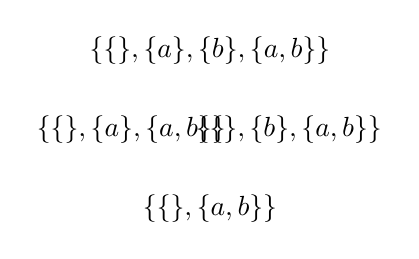
\begin{tikzpicture}
    \node (empty) at (0,0) {$\{\{\},\{a,b\}\}$};
    \node (a) at (-1,1) {$\{\{\},\{a\},\{a,b\}\}$};
    \node (b) at (1,1)  {$\{\{\},\{b\},\{a,b\}\}$};
    \node (all) at (0,2) {$\{\{\},\{a\},\{b\},\{a,b\}\}$};
  \end{tikzpicture}
\end{center}
\ss{13.3}
\ss{13.4}
\ss{13.5}
\s{16}
\ss{16.1}
\ss{16.2}
\ss{16.3}
\ss{16.8}
\s{17}
\ss{17.1}
\ss{17.2}
\ss{17.5}
\ss{17.6}
\ss{17.7}
\ss{17.10}
\ss{17.14}
\ss{17.15}
\ss{17.19}
\end{document}
